\chapter{Introduction}
\label{chapter1}

Climate change calls for a shift to renewable energy and restructuring of the electricity sector.
Sources \cite{eurostat2020} show as of the time of reading this paper, 44 \% of produced electricity in Europe was from combustible sources such as gas, fuel, and coal. Even 
though that is a significant decrease of 10 \% in the last 10 years, it is a significant Co2 emitter.
The same source \cite{eurostat2020} also states that a third of energy is consumed by the residential sector. It is estimated, 
that the human population will reach 10 billion inhabitants in the next 10 years, and ever-increasing ownership of electrical appliances such as smartphones, HVACs, and EVs will further elevate this issue.
Acknowledging this, reducing consumption in the residential sector could leave a significant impact on the human footprint. 

%increased time spent indoors*

The EU aims to be climate neutral by 2050, therefore it seeks to improve the efficiency of every part of pollution contributors through The European Green Deal.
A large part of these contributors is the Energy sector.
A subpart of the energy sector is the residential sector, where many advancements could be made to help to reach the goal.  

This could be achieved through various applications and methods that use load profiling as their core technology.
Authors in \cite{Chuan2014} proposed a method to reduce peak loads by studying consumer
appliance usage patterns. Paper \cite{Csoknyai2019} studied consumer usage patterns, and returned feedback that contributed to reducing consumption.
Another notable way is the use of distributed energy resources and managing them in such a way as to decrease the net output of energy flow such as the authors describe in
\cite{MORENOJARAMILLO2021445}. All described methods would reduce and alleviate the load off the power grid.

Load profiling in building energy consumption is not a novelty and had been in research since the 1980s.
While it was thought that aggregated LPs of households are relatively predictable, recent data obtained using smart meter data showed large deviance from user to user due to different lifestyles, as the author states in \cite{Review2021}.
In recent years LPs have changed due to renewable energy accelerated development of distributed energy resources such as residential photovoltaic
power plants, home wind energy, and using EVs with home batteries. Socioeconomic changes such as work-from-home, also drastically reshaped the LP curve. 

The thesis aims to propose and develop new, previously unused LPs, that will contribute to mitigating the raised issues. 

% finishing words here 

\section{Definition and types of LPs}
\label{sec:LP_types}
Author \cite{Review2021} defines terms as following:

\begin{itemize}
	\item Load: the electricity that all the electricity-powered devices in the household consume in unit time.
	\item Profile: a graph representing the significant features of the electricity load over time.
\end{itemize}

While the most commonly used feature is power, there are other derivatives such as the number of activations of an appliance or operating time.
Commonly, LP is a term used to describe the power consumption of a building.
That is not always the case, since the LP can be used to describe appliance-level consumption as well. 

The most common way LPs are presented is a daily power consumption profile such as shown in Figure \ref{fig:daily_power_profile}. 
While the graph is a sketch, it still presents a standard LP with morning and evening peaks.

\begin{figure}[H]
	\centering
	\caption{Average daily usage profile for an appliance or a building}
	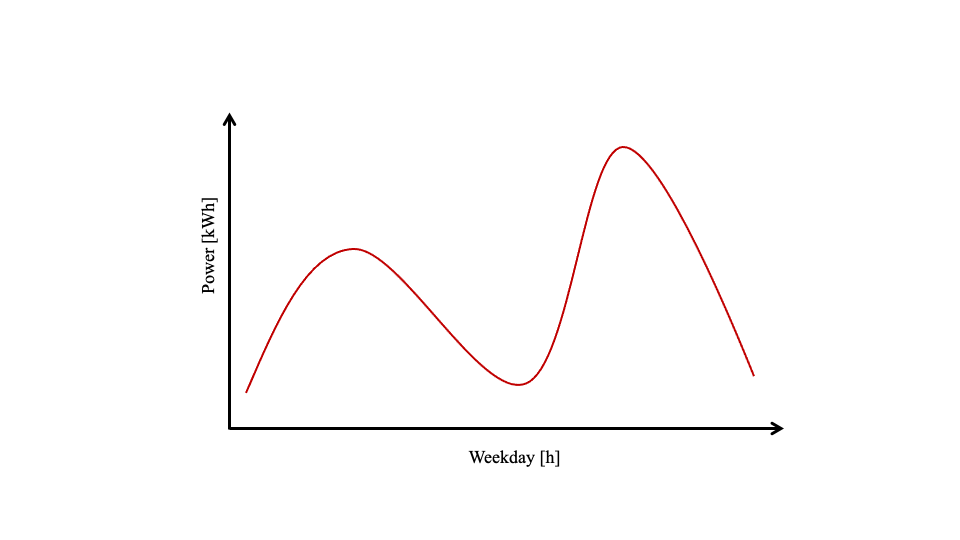
\includegraphics[width=0.9\textwidth]{Figures/profile_sketches/Slide1.png}
	\label{fig:daily_power_profile}
\end{figure}

Alternatively, we can use a histogram-based presentation such as can be seen in Figure \ref{fig:daily_act_profile}.
While Figure \ref{fig:daily_act_profile} presents the same data as Figure \ref{fig:daily_power_profile},
due to data processing, it could potentially reveal more relevant consumption patterns.

\begin{figure}[H]
	\centering
	\caption{Histogram of daily activations profile for an appliance or a building}
	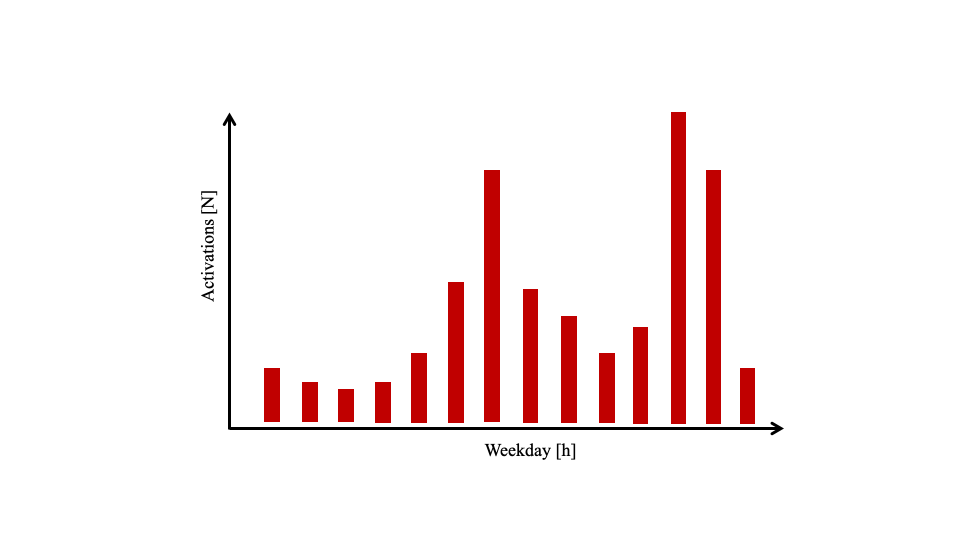
\includegraphics[width=0.9\textwidth]{Figures/profile_sketches/Slide5.png}
	\label{fig:daily_act_profile}
\end{figure}

All LPs can present whole-house usage or per-device usage. Each presentation has its advantages and disadvantages. 
To present more information sub-meter data can be used to represent whole-house usage with per-appliance contributions.
Such as on Figure \ref{fig:daily_act_m_profile} and \ref{fig:daily_power_m_profile}.

\begin{figure}[H]
	\centering
	\caption{Histogram of daily activations profile for appliance A and B}
	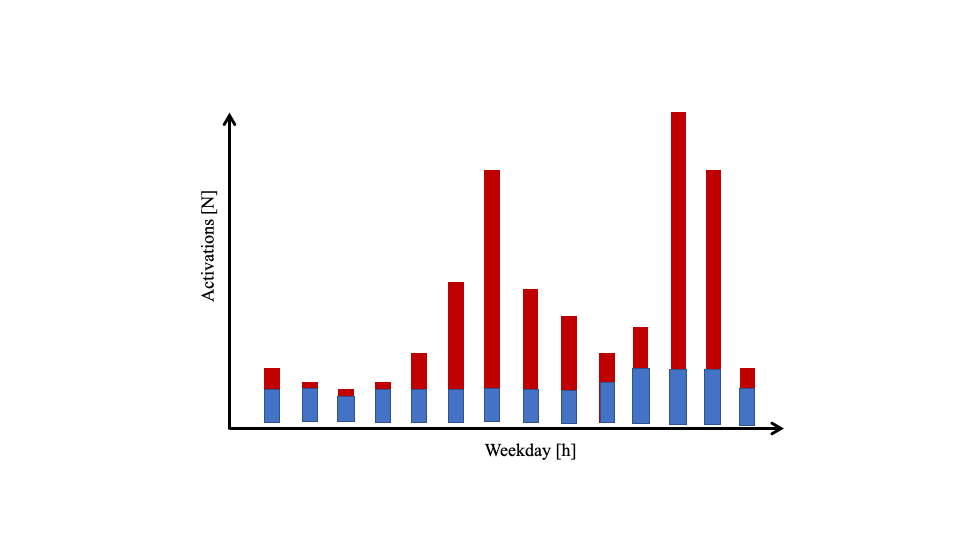
\includegraphics[width=0.9\textwidth]{Figures/profile_sketches/Slide8.png}
	\label{fig:daily_act_m_profile}
\end{figure}
\begin{figure}[H]
	\centering
	\caption{Average weekday power consumption for appliances A, B and C}
	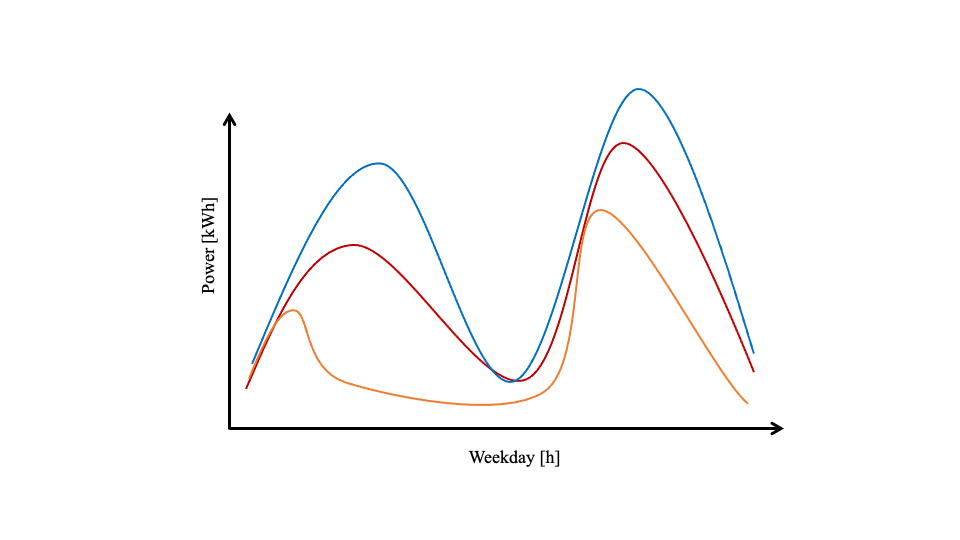
\includegraphics[width=0.9\textwidth]{Figures/profile_sketches/Slide2.png}
	\label{fig:daily_power_m_profile}
\end{figure}

To present as much information as possible all the above-mentioned attributes 
can be presented in a multidimensional way such as shown in Figure \ref{fig:heatmap_2dtime} and \ref{fig:heatmap_all_appl}.

\begin{figure}[H]
	\centering
	\caption{Number of daily activations/power consumption of one appliance/house in one-month period}
	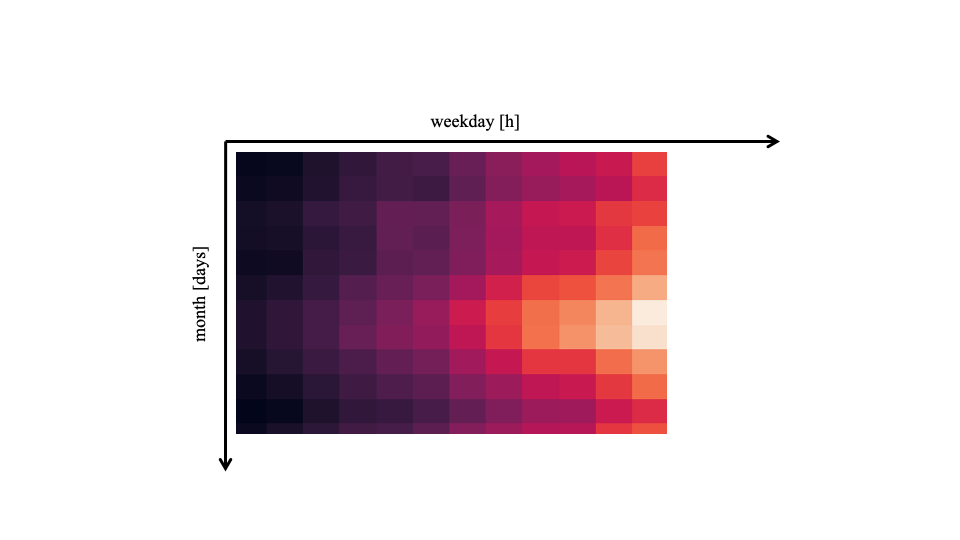
\includegraphics[width=0.9\textwidth]{Figures/profile_sketches/Slide10.png}
	\label{fig:heatmap_2dtime}
\end{figure}

Figure \ref{fig:heatmap_2dtime} presents a sketch and the heatmap does not present the real-world data. 
Even though, it is still possible to see that the plot presents one month of data, where we can see the consumption throughout each day.
The brightness presents the activity of the household or an appliance. 
The brighter the plot, the more activity for that hour of that day of the month.

One other thing to keep in mind when reading a such profile is that the origin is placed in the upper left corner.
This originates from image processing standards.

\begin{figure}[H]
	\centering
	\caption{Number of activations/power consumption for each appliance in one-month period}
	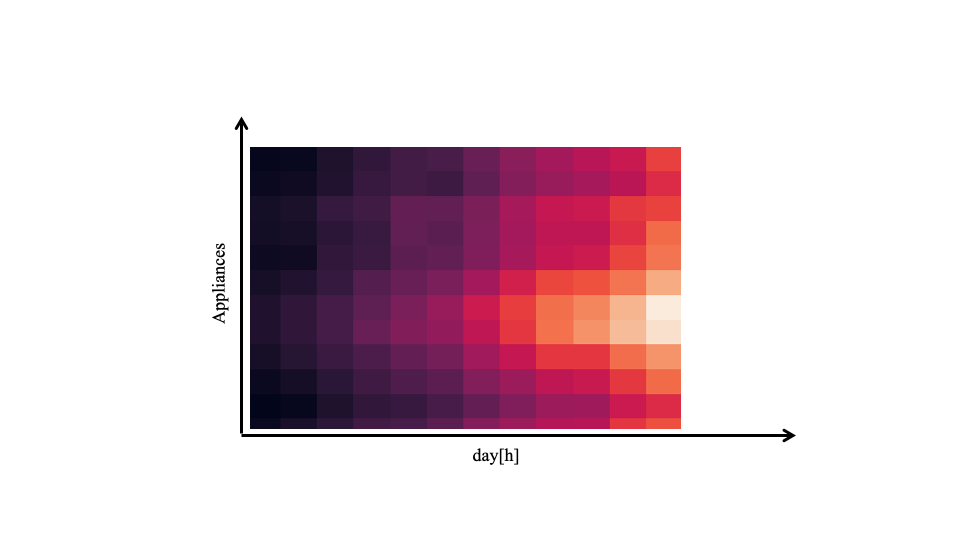
\includegraphics[width=0.9\textwidth]{Figures/profile_sketches/Slide12.png}
	\label{fig:heatmap_all_appl}
\end{figure}

Instead of having two-time axes, we could use one axis for different appliances in a household. 
Such example is Figure \ref{fig:heatmap_all_appl}.
In this case, we plot the consumption throughout the day on an x-axis, and a y-axis is used to display this for each appliance.

\section{LP use-cases}
\label{sec:use_cases_tree}

\begin{figure}[H]
	% \caption{General classification of LP use-cases}
	\label{tree:clasification_of_use_cases}
	\Tree[.{LP Use\ Cases} 
	[.Grid\\Managment Energy\\saving Zero\\Energy\\Buildings Demand\\response ]
	[.Anomaly\\Detection Elderly\\Care Fault\\Detection ]
	[.Other Develo-\\pment\\Feedback Occupancy\\Detection Energy\\Stealing ]
		]
\end{figure}

The load profiling method has a lot of different use cases across different fields.
In our case, we will split use cases into three classes.

The first class is grid management.
For example, it can be used to save energy by studying users' usage patterns and returning feedback, with suggestions on how to improve consumption.
In cases where buildings have grid batteries and PV installed, the same feedback could be used to minimize the amount of energy being pulled from the grid.
These are so-called zero-energy buildings (ZEB).
Electrical energy providers could use demand response programs in combination with the LPs to optimize the management of the grid, with minimal impact on users' daily lives.

The second class is anomaly detection.
The load profiles could be used to help the elderly in case of an accident or even help prevent one. 
They could be used to detect all kinds of early malfunctions in the operation of appliances, which would reduce service costs and save energy.

The last class is other, where occupancy detection, development feedback and energy stealing are all cases where LPs could be used. 

A more detailed description of each use-case with publications will be addressed in the next chapter in section \ref{sec:use-cases}


\section{Contributions}
\label{sec:contributions} % Change X to a consecutive number; for referencing this chapter elsewhere, use \ref{ChapterX}

The main goal of the master's thesis is to propose suitable LPs for supporting residential building consumption optimization and elderly care management.
To achieve this goal, we propose the following steps, where each step is a contribution to the scientific community.

\begin{enumerate}
	\item Surveying the state-of-the-art LPs (\ref{chapter2})
	\item Development of multidimensional activation LPs (ALP's) (\ref{chapter4})
	\item Visual analysis of ALP's (\ref{chapter5})
	\item Propose a new anomaly detection method for elderly care (\ref{chapter6})
\end{enumerate}


The first contribution will be provided by taking a look at existing research and use-cases. 
Using the publications, a table of profiles will be constructed.
The table will provide an overview of existing work, and reveal the gaps with LPs that were not yet utilized.
Using the related work we will try to determine in what field each LP could be used. 
While we will fill some gaps, many will be left open for fellow researchers to pursue.  

The second contribution will be provided in chapter \ref{chapter4}.
Here we will offer an in-depth look into the LPs, by presenting the profiles and showing how they present the consumption patterns.
Each LP presents a different pattern and therefore has a different use case. 

The third contribution will be provided in chapter \ref{chapter5}.
Here, we will use the t-SNE dimensionality reduction algorithm to show how samples are related.
By doing that we will obtain an understanding of the content that the datasets hold.

This newly found knowledge should help us provide the last contribution.
It will be provided in chapter \ref{chapter6}.
Here, we will design and construct elderly care assisted living system by utilizing one of the proposed profiles.
The system will be able to detect anomalies in the daily routine of the elder.
It should be simple, efficient and ready for real-world use.
With that, we should be able to prove that the LP can be efficiently utilized,
thus achieving the main goal of this thesis.


